\documentclass[UTF8]{article}
\usepackage{bm}
\usepackage{amsmath}
\usepackage{cases}
\usepackage{cite}
\usepackage{graphicx}
\usepackage[margin=1in]{geometry}
\geometry{a4paper}
\usepackage{fancyhdr}
\usepackage{array}
\pagestyle{fancy}
\usepackage{wrapfig}
\fancyhf{}
\usepackage{float}  %设置图片浮动位置的宏包
\usepackage{subfigure}
\usepackage{caption}
\usepackage{booktabs}
\usepackage{listings}
\usepackage{xcolor}
\usepackage{multirow}
\lstset{numbers=left, %设置行号位置
	numberstyle=\tiny, %设置行号大小
	keywordstyle=\color{blue}, %设置关键字颜色
	commentstyle=\color[cmyk]{1,0,1,0}, %设置注释颜色
	frame=single, %设置边框格式
	escapeinside=``, %逃逸字符(1左面的键),用于显示中文
	breaklines, %自动折行
	extendedchars=false, %解决代码跨页时,章节标题,页眉等汉字不显示的问题
	xleftmargin=2em,xrightmargin=2em, aboveskip=1em, %设置边距
	tabsize=4, %设置tab空格数
	showspaces=false %不显示空格
}

\title{Characteristics of Gratings and Measurement of Wavelengths of Light Waves}
\author{by 22 Artificial Intelligence ChenxuZhang}
\date{2023.12.10}
\pagenumbering{arabic}
\begin{document}
	\fancyhead[L]{ChenxuZhang}
	\fancyhead[R]{ID 202264691028}
	\fancyfoot[C]{\thepage}
	
	\maketitle
	\tableofcontents
	\newpage
	
	\section{Abstract}
In 1881, the American physicist Albert Abrham Michlson (1852-1931) designed an interferometric device, the Michlson interferometer, to measure the speed of light on the basis of the principle of interference between two beams of light generated by splitting the amplitude. With this instrument, Michaelson Morley (1838-1923) completed the "Ether" drift experiment, which is of great significance in the theory of relativity, and completely denied the existence of the "Ether", thus providing an experimental basis for the theory of relativity proposed by Albert Einstein. The Michaelisen interferometer is capable of measuring the Ether at very high speeds. The Michelson interferometer can measure small changes in length with high precision, and can observe and analyze various interference phenomena.

In spectroscopy, Michaelson used the interferometer designed by him to discover the ultra-fine structure of the hydrogen spectrum, as well as mercury and thallium spectra, laying the theoretical and experimental foundation for the development of modern atomic spectroscopy, molecular spectroscopy and laser spectroscopy and other disciplines. In metrology, Michaelson found that the length of the international meter proton that 1 meter is equal to 1553163.5 times the wavelength of the red cadmium spectral line (6438.4722A), the International Bureau of Weights and Measures decided to cadmium wavelength determination of the length of the international meter proton, Michaelson's work for the length of the unified benchmark for human beings to obtain the foundation. Because of the contribution of Michelson to optical precision instruments, as well as used in spectroscopy and metrology research, so won the Nobel Prize in Physics in 1907.

	\section{Purpose of the experiment}

   $\bm{A}$.Understand the structure, principle and adjustment of the Michelson interferometer.\\
   $\bm{B}$.Observation of non-dimensional interference phenomena in point light sources and isotropic and isothickness interference in extended light sources.\\
   $\bm{C}$.Measuring the wavelength of He-Ne lasers with a Michelson interferometer.\\
   $\bm{D}$.Determination of the wavelength difference between the yellow double lines of sodium lamps using isochronous interference fringes.


	\section{Experimental apparatus}
	Michelson interferometer, He-Ne laser, low-pressure sodium lamp, beam expander, viewing screen, etc.

\begin{figure}[h]
    \centering
    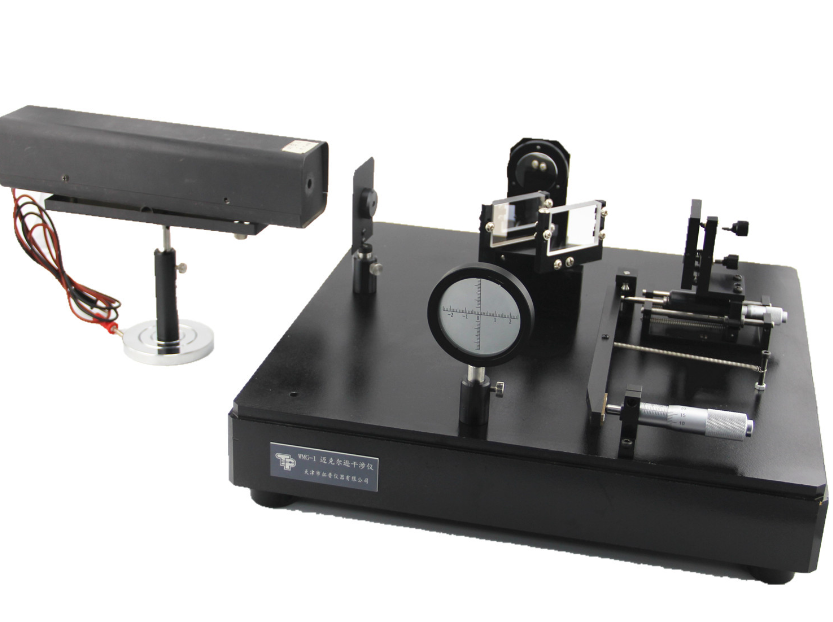
\includegraphics[width=0.5\linewidth]{FIG2.png}
    \caption{Michelson interferometer}
    \label{fig:Michelson interferometer}
\end{figure}

\begin{itemize}
    \item \textbf{Michelson Interferometer:} A precision optical instrument used for interferometry, consisting of a beam splitter, mirrors, and other components to study the interference of light waves.
    
    \item \textbf{He-Ne Laser:} A helium-neon laser emitting visible red light commonly used in various optical experiments and applications.

    \item \textbf{Low-Pressure Sodium Lamp:} A lamp that produces light by exciting sodium vapor at low pressure, emitting characteristic yellow-orange light often used for specific spectral studies.

    \item \textbf{Beam Expander:} An optical device designed to increase the diameter of a laser beam, enhancing its spatial coherence and facilitating precise measurements.

    \item \textbf{Viewing Screen:} A surface where the interference patterns or optical phenomena can be observed and analyzed visually.

    % Add more items as needed
    
\end{itemize}


\begin{figure}[h]
    \centering
    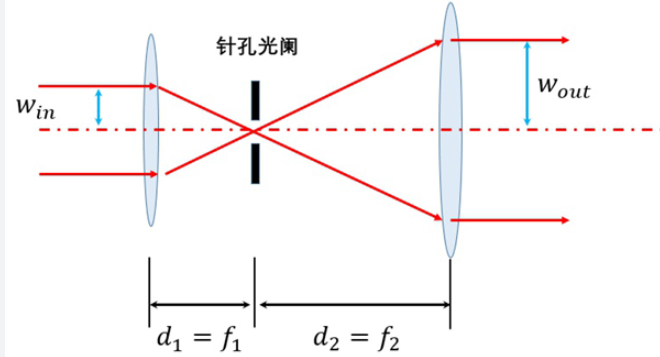
\includegraphics[width=0.5\linewidth]{FIG3.png}
    \caption{beam expander}
    \label{fig:beam expander}
\end{figure}

        
	\section{Method}
 Mackelson interferometer in modern physics and measurement technology has a wide range of applications, such as it can measure the wavelength of light waves, tiny length, the coherence of the light source length, etc., if the coherence of the light source with better, but also for the larger length of the precise measurement, and it can be used to study the temperature, the pressure on the propagation of light and other effects.
	
 \subsection{Optical path principle}
\begin{figure}[h]
     \centering
     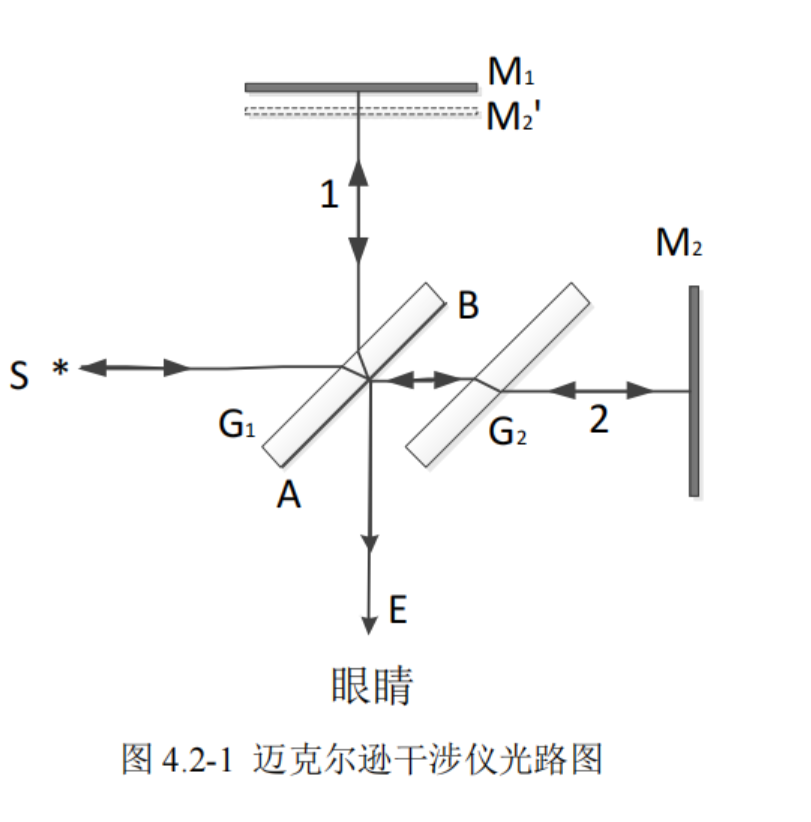
\includegraphics[width=0.5\linewidth]{FIG.png}
     \caption{Michelson interferometer optical path diagram}
 \end{figure}
 
The optical path of the Michaelisen interferometer is shown in Fig. 4.2-1. The beam emitted from the light source S is incident on the beamsplitter plate G1, the rear surface of the G1 plate is coated with a semi-transparent metal film AB (silver-plated or aluminum-plated), which splits the incident light into the reflected light 1 and transmitted light 2 of approximately equal intensity, and these two beams of light are respectively directed perpendicularly to the mirrors M1 and M2, and then returned to the rear surface of the G1 after the reflections of M1 and M2 along the original optical path to transmit and reflect the light along the two beams of light propagating along the E direction to produce convergence. The two beams of light propagating along the direction of E converge, and since the two beams of light have the same frequency, the same direction of vibration and a constant phase difference (i.e., the conditions for interference are met), interference is formed. In order to compensate for the extra distance traveled by beam No. 1 in the optical path, a compensation plate G2 is inserted between the optical path G1 and the mirror M2. The material properties, geometry, and thickness of the G2 plate are the same as those of G1, and the direction is parallel to that of the G1 plate.\\
 
 When the eye looks at the G1 plate from point E, in addition to the image produced by the M1 mirror on the light source, it also sees the reflected image of M2 in G1, M2'. To the observer, the interference caused by the reflections of M1 and M2 can be seen as interference caused by light reflected from the upper and lower surfaces of the air layer between M1 and M2'. The advantage of this is that M2' is not a physical object, so that it can be discussed in terms of thin-film interference by arbitrarily changing the position of M1 or M2 so that M2' is in front of or behind M1, or so that they intersect, or so that they are completely overlapping and parallel.

   \subsection{Non-deterministic interference from a point light source}

\begin{figure}[h]
    \centering
    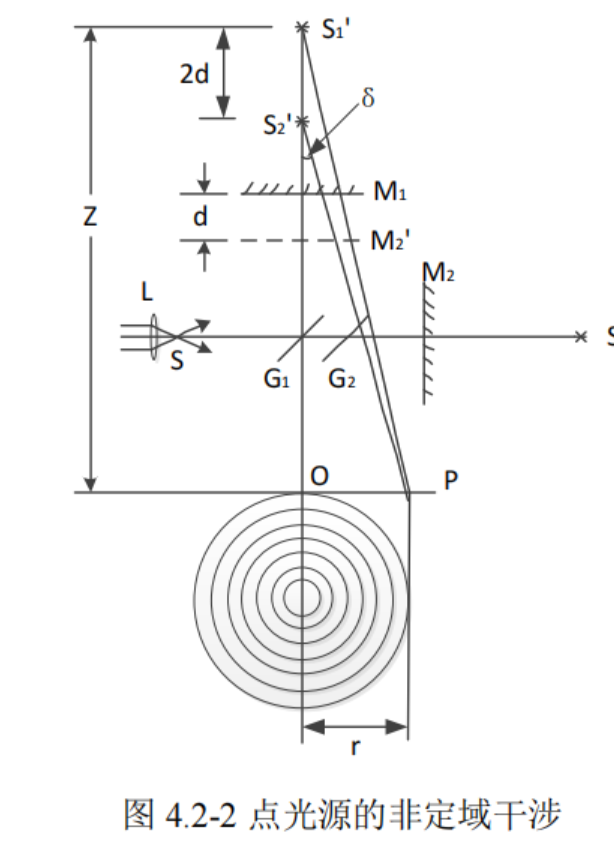
\includegraphics[width=0.5\linewidth]{FIG4.png}
    \caption{Non-deterministic interference of point light sources}
\end{figure}
A laser can be used as a light source to observe the non-deterministic interference phenomena of the Michelson interferometer. As shown in Fig. 4.2-2, the laser beam is converged into a very bright point light source S by a short focal length lens L, and is directed to the Michelson interferometer. the point light source is reflected by plane mirrors $M_1$ and $M_2$, and is equivalent to the coherent beams emitted by two point light sources $S'_1$ and $S'_2$. $S'$ is the equivalent light source of S, which is the virtual image formed by the semi-reflective surface $G_1$, $S'_1$ is the virtual image formed by S' through $M_1$, and $S'_2$ is the virtual image formed by S' through $M'_2$. Figure 4.2-2 shows that as long as the observation screen is placed in the overlapping area of the light waves from the two point sources, the interference phenomenon can be seen, so this interference is called non-deterministic interference.\\

If observed perpendicular to the $S'_1$ $S'_2$ line, a set of concentric circles can be seen, and the center of the circles is the $S'_1$ $S'_2$ line and the focal point of the observation screen O. Since the points on the same level of secondary interference fringes have the same angle of inclination to the virtual light source, the interference fringes are also called point source isotropic interference fringes. Because the points on the same level of interference fringe have the same inclination to the virtual light source, this interference fringe is also known as the point source of equal inclination interference fringe.\\

As you can see from the graph:\\
        \[ \alpha = 2d\cos \delta \approx 2d(1-\frac{1}{2}\delta ^{2})\]\\
   
 If the incident light is monochromatic and has a wavelength of $\lambda$ , the positions of the light and dark interference fringes on the viewing screen satisfy the following conditions:\\

 \[ \alpha =2d\cos \delta =\begin{cases}  k\lambda & (light)\\  (2k+1)\lambda /2& (dark)\end{cases} \]\\
   
The wavelength of the light wave $\lambda$ can be measured from the above equation by reading from the instrument and counting the number of stripe changes N. If $\lambda$ is taken as the standard value and the distance moved by $M_1$ is measured when N rings are emerging or disappearing, the error of the instrument transmission system can be corrected by comparing it with the theoretical value calculated by the formula.

   \subsection{Fixed-field interference with extended light sources}

\begin{figure}[h]
    \centering
    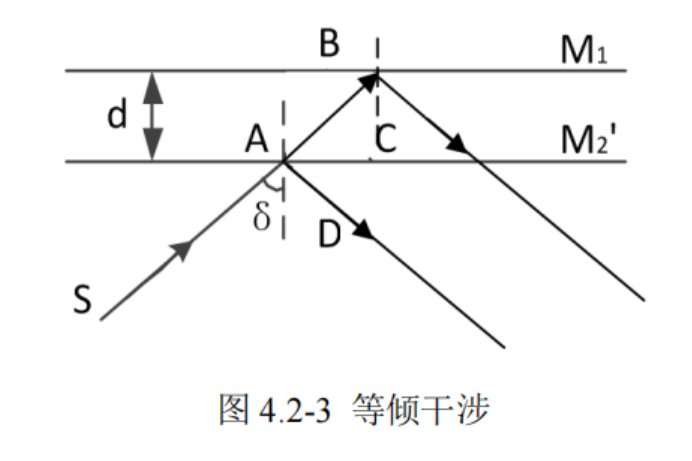
\includegraphics[width=0.5\linewidth]{FIG5.png}
    \caption{isochronous interference}
\end{figure}
   \subsubsection{Isochronous interference}
Adjust the reflector M1 and reflector $M_2$ of the Michelson interferometer to be perpendicular to each other, i.e., $M_1$ and $M'_2$ are parallel to each other. This is shown in Fig. 4.2-3. The light emitted from a point S on the surface light source, the angle of incidence is $\delta$, after the reflection of $M_1$ and $M'_2$ into two beams of light parallel to each other, the discussion of their optical range difference is similar to the results of the point source of non-stereotypical interference, i.e.\\

\[ \alpha =(\overline{AB}+\overline{BC} )-\overline{AD}=2d\cos\delta \] \\

On a surface light source, there are countless points S incident at the same angle of incidence $\delta$, after reflection, they are parallel to each other, they meet at infinity and produce interference, and a set of concentric interference fringes can also be seen by eye observation. Only these fringes can only occur in a specific region of space, so it is called fixed interference. At the same time, each point of light for different angles of incidence, the level of interference fringes are different, so it is called isotropic fixed interference.

\begin{figure}
    \centering
    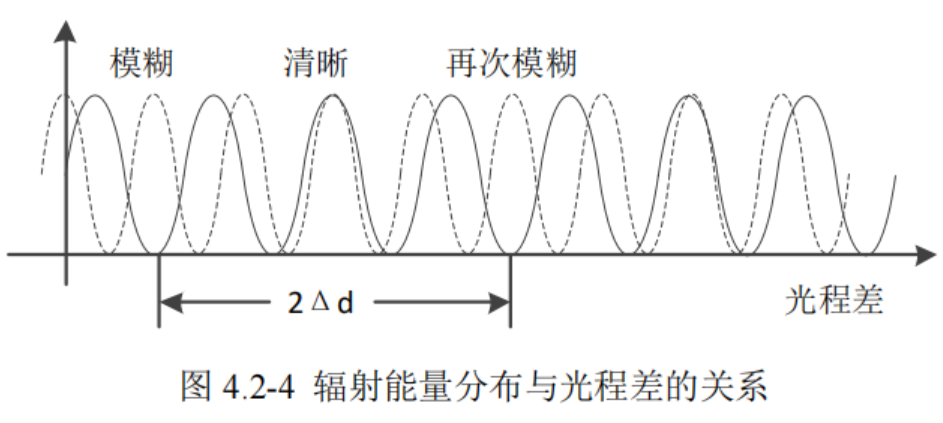
\includegraphics[width=0.5\linewidth]{FIG6.png}
    \caption{Enter Caption}
\end{figure}

The yellow light of a sodium lamp consists of two spectral lines with similar wavelengths: $\lambda_1=588.996nm$ and $\lambda_2=589.593nm$, and the difference in wavelengths can be measured using a Michelson interferometer. When observing their isotropic interference fringes, if the $k_1$ bright fringe of $\lambda_2$ and the $k_2$ dark fringe of $\lambda_1$ appear at the same time in the center of the isotropic interference circular fringe, then the optical range difference is:\\

\[\alpha =2d=k_{1}\lambda _{2} = (k_{2}+\frac{1}{2}  )\lambda _{1} \]\\

In this case, the bright stripes of $\lambda_2$ light overlap with the dark stripes of $\lambda_1$ light, and the sum of the radiant energy distributions of the two light waves is almost the same everywhere, causing the stripes to blur in the field of view. If you move $M_1$, you can see that the stripes gradually become clear again. When the two bright stripes of $\lambda_1$ and $\lambda_2$ light overlap, the sum of the radiant energy distributions of the two light waves has the greatest contrast, and the stripes in the field of view are the clearest. If we continue to move $M_1$ in the same direction, we can see that the stripes in the field of view become less and less clear. When the bright stripes of $\lambda_2$ light and the dark stripes of $\lambda_1$ light overlap again, the stripes in the field of view are blurred again. This process can be illustrated by the relationship between the radiant energy distribution of $\lambda_1$ light and $\lambda_2$ light and the optical range difference, as shown in Fig. 4.2-4. The optical range difference due to the $M_1$ shift is exactly satisfied when these two blurring occurs:\\

\[k\lambda _{2} =(k+1)\lambda _{1}\]\\ 

Thus the wavelength difference of the sodium double line:\\

\[\Delta \lambda =\frac{\overline{{\lambda^{2}  } } }{2\Delta d^{'} }\]\\

Therefore, it is only necessary to measure $\Delta d^{'}$ to measure the wavelength difference between the sodium double lines.
	
 \subsubsection{equal-thickness interference}
When $M_1$ and $M_2$ are not perpendicular, that is, $M_1$ and $M'_2$ are not parallel, but have a very small angle θ, between $M_1$ and $M'_2$ is equivalent to an air splitting tip, with an extended source of light irradiation, there will be an equal-thickness interference fringes, which are localized in the vicinity of the air splitting tip. Since the angle θ is very small, the optical range difference can still be calculated by equation (4.2-1), so the equal-thickness interference is actually a kind of interference related to the inclination angle and the thickness of the air layer.

\begin{figure}
    \centering
    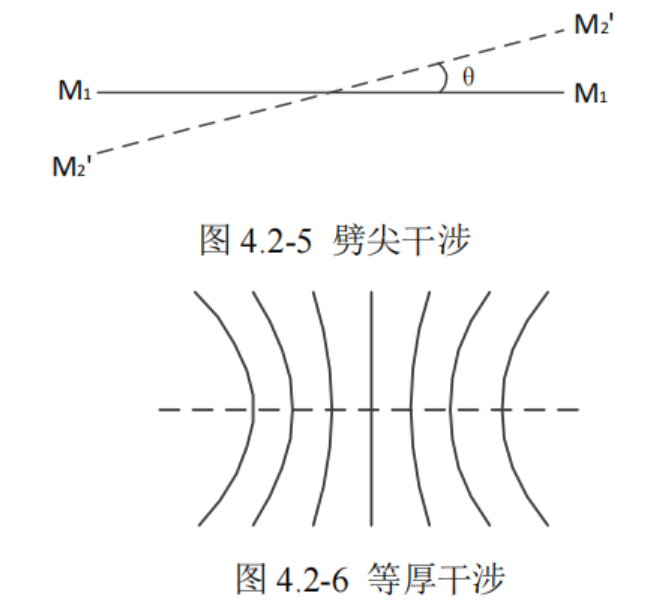
\includegraphics[width=0.5\linewidth]{FIG7.png}
    \caption{Split-tip interference and equal-thickness interference}
\end{figure}

When $M_1$ and $M'_2$ intersect, $d=0$ on the intersection line, then $\alpha=0$. Considering the half-wave loss when the light is reflected at the different interfaces of the air splitting tips, there is a dark interference at the intersection line, which is called the central stripe. On both sides of the intersection line are two top-to-top split-tip interference, as shown in Fig. 4.2-5. When the angle $\theta$ is very small, the interference fringe near the intersection line can be approximated as a straight line, parallel to the central dark fringe. Farther away from the central stripe, the interference fringes are bent due to the influence of the incident angle δ. As the viewing angle $\delta$ increases, $\theta$ does not change (i.e., the optical range of the same sub-stripe remains constant), and d must be increased to make the observed sub-stripe concave to the sides, as shown in Figure 4.2-6.\\

When irradiated with white light, a variety of different wavelengths of light produced by the interference fringe light and dark superimposed on each other, generally do not appear interference fringe. Only in the intersection line of $M_1$ and $M'_2$, for various wavelengths of light, the optical range difference is $\theta /2$(additional when reflecting$\theta /2$), so it produces straight line black stripes, that is, the so-called central stripes, with symmetrically distributed color stripes on both sides. d is a little larger, because of the various wavelengths of light, to meet the conditions of dark and light stripes are different, the interference fringes produced by the dark and light overlap with each other, and as a result, it does not show the fringes to. The result is that no fringes are visible. The central stripe can only be determined with white light, and the position of $d=0$ can be determined from this point.

 After the central stripe appears in the field of view, a transparent object with refractive index $n_x$ and thickness D is placed between M1 and A. Then the two beams of light appear Optical range difference $\alpha$ :\\
 
 \[\alpha =2D(n_{x}-n_{o} )\]\\

 If the thickness D of the transparent object is known, the refractive index $n_x$ of the transparent object can be measured by the above formula; conversely, if the refractive index of the transparent object is known, the thickness D of the transparent object to be measured can be calculated.

 
 \section{Procedure}
 Special reminder, the Michelson interferometer is a precision optical instrument, must be careful when adjusting, can not touch the surface of the reflector, beam splitter, compensation plate and other optical devices with hands during the experiment.
	\subsection{Adjustment of the Michelson interferometer}

 \begin{itemize}
	\item Familiarize yourself with the structure of a Michelson interferometer. Adjust the height of the light source so that the light source is approximately the same height as the beam splitter and is oriented at an angle of 45 degrees to the beam splitter.
	\item Adjust the optical range difference. Adjust the rotation of the rough hand wheel so that the distances of the moving mirror $M_1$ and fixed mirror $M_2$ relative to the beamsplitter are approximately equal.
	\item Adjust the Michelson interferometer so that mirror $M_1$ and mirror $M_2$ are perpendicular to each other, i.e., $M_1$ and $M'_2$ are parallel to each other. The adjustment method varies slightly depending on the light source.\\
 For He-Ne lasers, optical screen 6 should be mounted and viewed on the optical screen. Turn on the laser, so that the laser is basically perpendicular to the $M_2$ surface, in front of the light source to put a small hole diaphragm, adjust the two screws on the $M_2$ (sometimes also need to adjust the two screws behind the $M_1$), so that the laser beam emitted from the small hole, through the $M_1$ and $M_2$ reflection in the hairy glass after the overlap, then you can see the two rows of light on the hairy glass one by one coincide. Remove the small aperture diaphragm, replaced by a short focal length lens and make the light source into a diffuse beam, in the two beam range difference is not too large, in the wool glass screen can be observed interference fringe, gently adjust the section of the $M_2$ section of the screws after the center should be basically in the center of the wool glass screen of the circular stripes.
	\end{itemize}


    \subsection{Measurement of laser or sodium wavelength}
   \begin{itemize}
	\item Keep the interferometer tuned. Turn the micrometer wheel in one direction until a continuous change in the interference fringes is observed (elimination of the headspace difference) and record the data. It should be noted that the micrometer wheel can only be turned in one direction during the entire test, not back and forth.
	\item For every 50 stripes "born" or "swallowed" by the center, the data should be recorded once, and the total number of N should not be less than 500, and the data should be processed to find out the value of $\lambda$ by the difference-by-difference method.
\end{itemize}

 \begin{figure}[h]
     \centering
     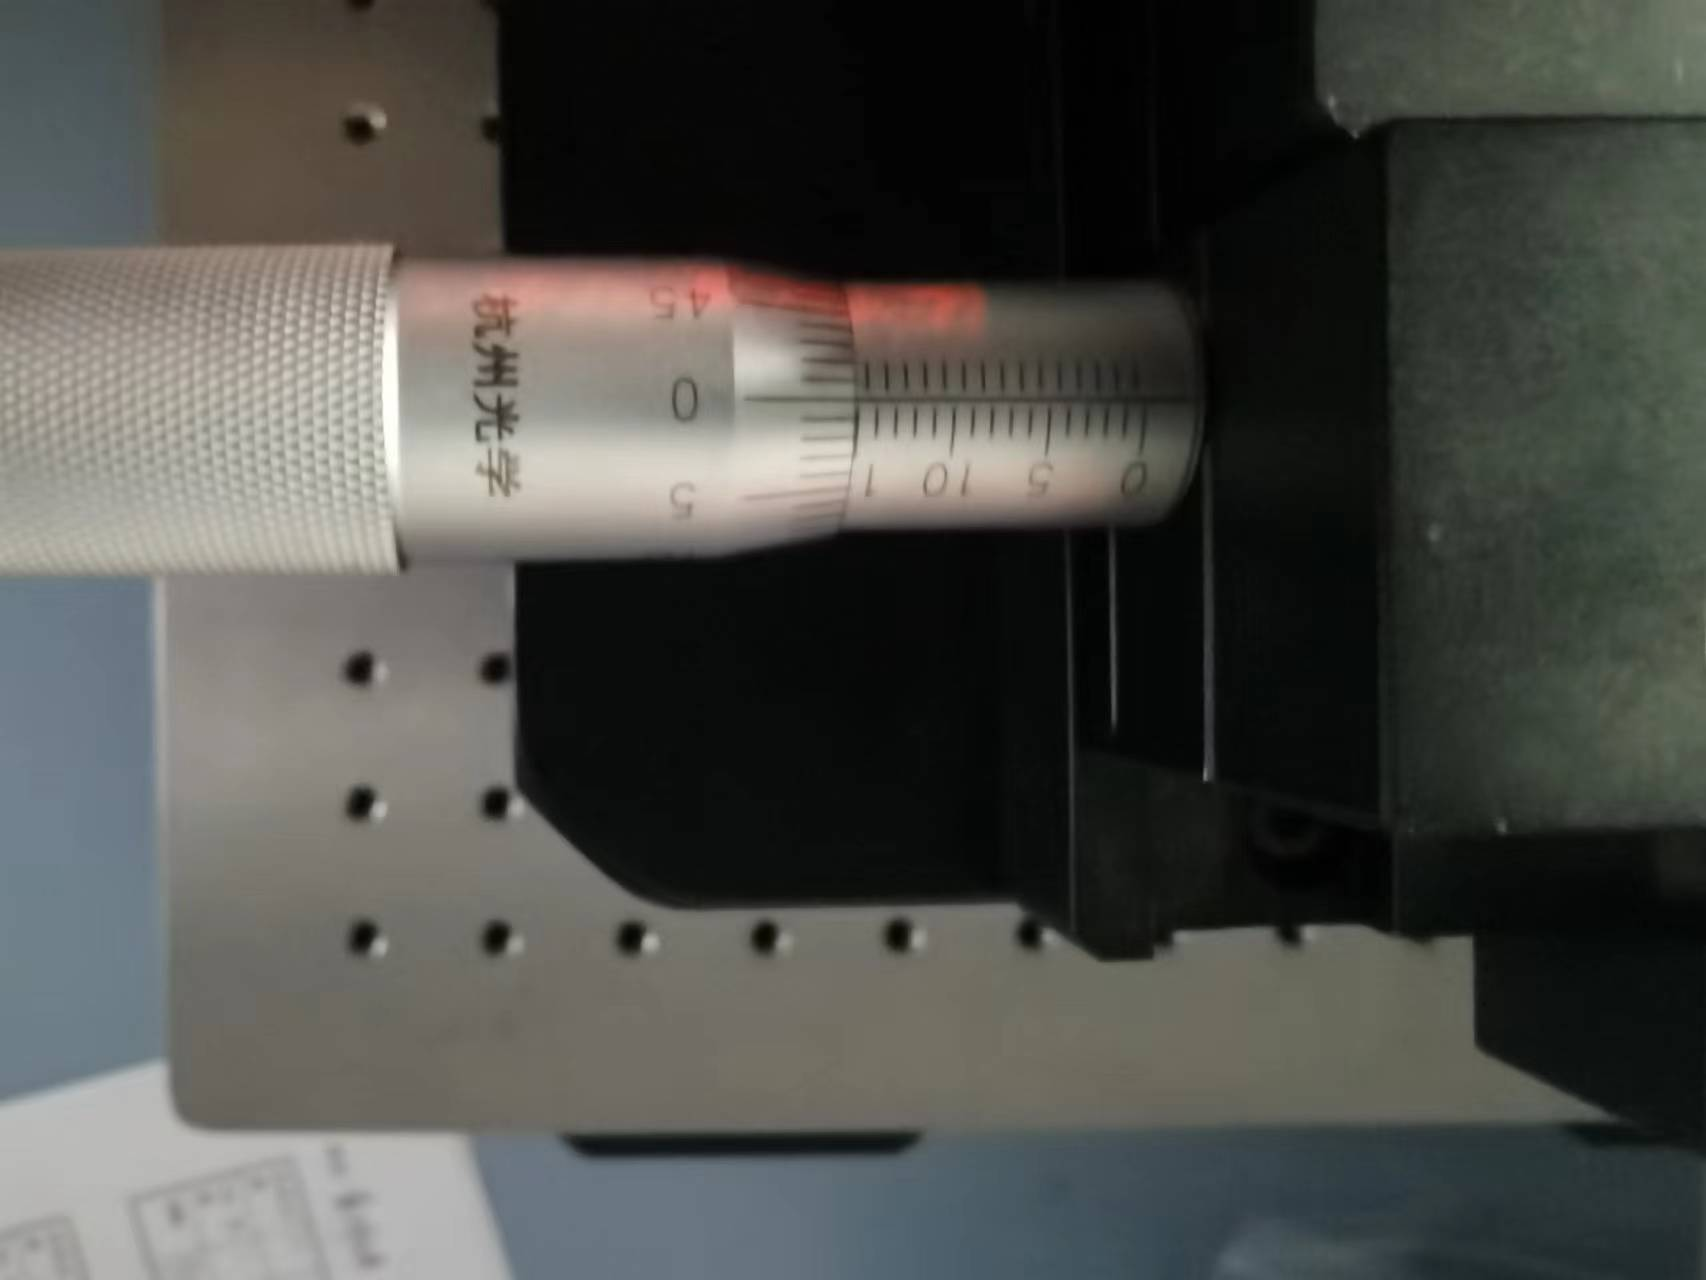
\includegraphics[width=0.5\linewidth]{FIG8.jpg}
     \caption{sodium wavelength}
     \label{fig:enter-label}
 \end{figure}

 
	\section{Original Data \& Analysis}
After experimental measurements, the relationships in Table 1 are obtained:\\

\begin{table}[H]
  \centering
  \caption{The relationship of the number of gushing stripes on the position of the moving mirror}
    \begin{tabular}{crrrrrrrr}
    \toprule[2pt]
    \multicolumn{1}{l}{number of changes} & 50 & 100 & 150 & 200 & 250 & 300 & 350 & 400  \\
    \midrule
    \multicolumn{1}{l}{position of $M_1$} & $X_1$ & $X_2$ & $X_3$ & $X_4$ & $X_5$ & $X_6$ & $X_7$ & $X_8$  \\
    reading& 19.825 & 18.764 & 16.720 & 15.115 & 13.531 & 11.952 & 10.307 & 8.685 \\
    \bottomrule[2pt]
    \end{tabular}%
  \label{tab:addlabel}%
\end{table}%

Plotting an image of the following table and approximating it with a straight line, we get the following image:\\

\begin{figure}[h]
    \centering
    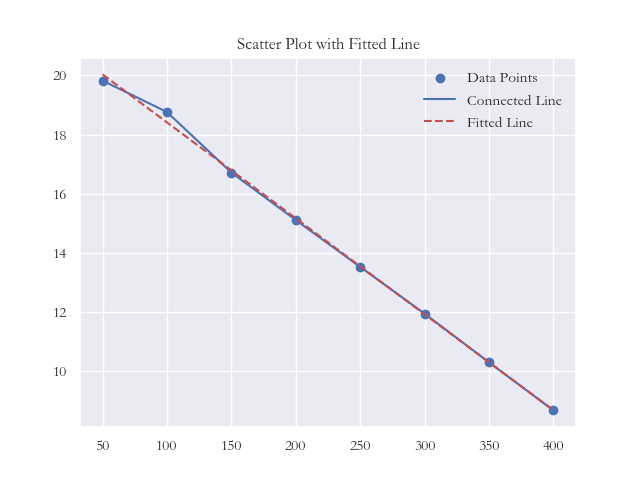
\includegraphics[width=0.9\linewidth]{FIG9.png}
    \caption{Plotting the scatterplot}
    \label{fig:enter-label}
\end{figure}

The equation obtained from the linear fitting:\\
\[y=-0.0324x+21.656\]\\

Using the differential method, then we cab obtain $\delta$ d:\\
\[\Delta d=\frac{\overline{d_{N+5} -d_N} }{5} =0.016018(mm)\]\\

From the previously mentioned formula:\\
\[\lambda =\frac{2\Delta d}{N} =0.000640725(mm)=640.725(nm)\]\\


	
 \section{Experimental conclusion and Error analysis}
	\subsection{Conclusion}

	\begin{itemize}
	\item Based on the above experiments, we finally obtained the experimental results: Wavelength of laser light produced by HeNe lasers is 640.725(nm) with small error.
	\item The wavelength measured by the experiment is clear, the data is accurate, and the results are normal, so the experiment is more successful.
	\item The principle of this experiment is relatively simple and there is no difficulty in operation. But attention should be paid to the accuracy of each measurement.
	\end{itemize}

	\subsection{Error analysis}
	After data comparison, this experiment may have some deviation compared with the standard experimental results, after analyzing the possible influencing factors as follows:
	\begin{itemize}
	\item If the output of a laser or other light source is unstable, this can lead to instability in the interference pattern, which can affect wavelength or coherence measurements.
	\item Errors may be introduced by the detector or measurement equipment used. For example, the sensitivity and resolution of the detector may limit the accuracy of the experiment.
	\item The angular adjustment of the beam splitter may not be precise enough, resulting in uneven beam splitting, which in turn affects the interference pattern.
	\end{itemize}

\begin{appendix}
 \section{Experimental data recording graph} 
     	 \begin{figure}[h]
     	     \centering
     	     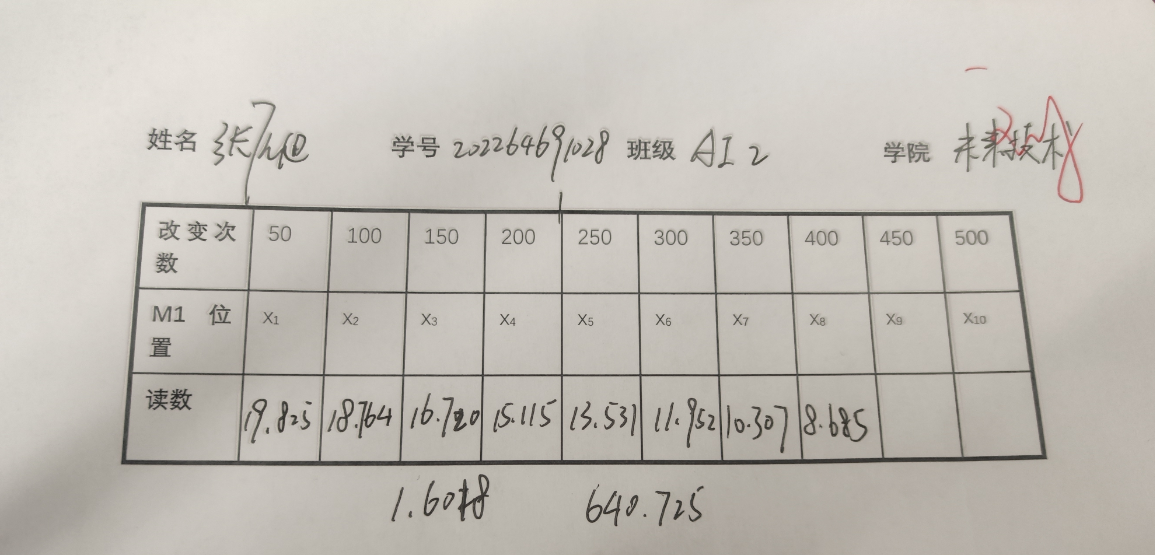
\includegraphics[width=0.8\linewidth]{FIG10.png}
     	     \caption{Experimental data recording graph}
     	     \label{fig:enter-label}
     	 \end{figure}
 \end{appendix} 

	
	
	\end{document}  